
\subsection{Ejercicios}
\begin{itemize}
 \item 
\textbf{Ejercicio 4}  Completar la implementación del scheduler Round-Robin implementando los
metodos de la clase SchedRR en los archivos sched rr.cpp y sched rr.h. La implementacion
recibe como primer parametro la cantidad de nucleos y a continuacion los valores de sus
respectivos quantums. Debe utilizar una unica cola global, permitiendo ası la migracion de
procesos entre nucleos.
\item \textbf{Ejercicio 5}Disene un lote con 3 tareas de tipo TaskCPU de 50 ciclos y 2 de tipo TaskConsola
con 5 llamadas bloqueantes de 3 ciclos de duracion cada una. Ejecutar y graficar la simulacion
utilizando el scheduler Round-Robin con quantum 2, 10 y 50.\\
Con un cambio de contexto de 2 ciclos y un solo nucleo calcular la latencia, el waiting
time y el tiempo total de ejecucion de las cinco tareas para cada quantum. 
¿En cual es mejor cada uno? ¿Por que ocurre esto?
\item \textbf{Ejercicio 6} Grafique el mismo lote de tareas del ejercicio anterior para el scheduler FCFS.
Haciendo referencia a lo que se observa en los graficos de este ejercicio y el anterior, explique
las diferencias entre un scheduler Round-Robin y un FCFS.
\item \textbf{Ejercicio 7} Grafique el mismo lote de tareas del ejercicio anterior para el scheduler FCFS.
Haciendo referencia a lo que se observa en los graficos de este ejercicio y el anterior, explique
las diferencias entre un scheduler Round-Robin y un FCFS.
\item \textbf{Ejercicio 8} Implemente un scheduler Round-Robin que no permita la migracion de procesos
entre nucleos (SchedRR2). La asignación de CPU se debe realizar en el momento en que se produce la carga 
de un proceso (load). El nucleo correspondiente a un nuevo proceso sera aquel
con menor cantidad de procesos activos totales (RUNNING + BLOCKED + READY).Explique un escenario real 
donde la migracion de nucleos sea beneficiosa y uno donde no (mencione
especificamente que metricas de comparacion vistas en la materia mejorarıan en cada caso).
Disene un lote de tareas en nuestro simulador que represente a cada uno de esos escenarios
y grafique su resultado para cada implementacion. Calcule y compare en cada grafico las
metrica que menciono.

\end{itemize}


\subsection{Resultados y Conclusiones}

\subsubsection[Resolución Ejercicio 4]{Ejercicio 4}
Para desarrollar la implementación del scheduler $Round-Robin$ y que este funcione de una forma correcta
utilizamos una serie de estructuras puntuales. \\
Las mismas son las siguientes:\\
\begin{enumerate}
 \item Una cola global, la cual nombramos $q$, esta contiene los $PID$ de los procesos activos que no estan
 bloqueados y en el tope de la misma se encuentra el próximo proceso a correr. Esta cola,
 fue desarrollada para que cuando se desaloje un proceso por finalizar su $quantum$ la misma pase al final de
 la cola y generando el ciclo acorde al comportamiento de este scheduler.
 \item Un vector denominado $cores$, este tiene en su elemento $i$ el pid correspondiente a
al proceso que está corriendo en el core $i+1$. Inicializamos todos los elementos en -1, esto
corresponde a la Idle Task, de esta forma reconocemos que no se cargaron procesos en los núcleos.
\item Un vector $quantum$ guarda en la posicion $i$ el quantum que se dispuso a cada núcleo.
\item Un vector $quantumActual$ aqui guardaremos la cantidad de ticks que le quedan al proceso
desde que fue cargado en el core.
\item Una lista de $bloqueados$ esta tendra procesos que se bloquearon cuando estaban corriendo.
\end{enumerate}

De esta manera, con estas estructuras nos permiten determinar para cada tarea, cuándo, y cuánto 
de su quantum consumieron de forma que podamos desalojarla correctamente.\\

A su vez, tomamos ciertas decisiones en esta implementación:
\begin{itemize}
 \item Si una tarea se encuentra bloqueada cuando se produce el tick del reloj, esta misma es desalojada
de la cola global, y agregada en un lista de bloqueados. Además, sera reseteado el quantum, se le
dará inicio a la próxima tarea que se encuentre ready y cuando el sistema operativo, nos envie una
señal de unblock, la tarea desalojada regresará al final de la cola global.

\end{itemize}


\subsubsection[Resolución Ejercicio 5]{Ejercicio 5}

EN ESTE PUNTO SIRVE TODO LO ESCRITO SOLO HAY Q CAMBIAR GRAFICOS!

\indent El algoritmo de scheduler \textbf{Round-Robin} tiene como caracter\'istica asignar a todas las tareas 
un determinado tiempo m\'aximo de procesamiento, a esto se lo llama $quantum$. \\
\indent Este tiempo esta definido para cada n\'ucleo en particular, dependiendo de en cu\'al de ellos est\'en 
ejecutando los procesos, se les asignar\'a el respectivo tiempo m\'aximo.\\
\indent Otra caracter\'istica del \textbf{Round-Robin} es que las tareas se encolan y se ejecutan c\'iclicamente. 
Osea que cuando se deja de ejecutar, si no termin\'o su ejecuci\'on, la tarea se encolar\'a al final de la lista. 
Como elecci\'on de diseño, elegimos que se use una cola global para todos los procesadores, aunque tambi\'en
se podr\'ia tener una cola para cada n\'ucleo. \\
\indent A su vez, tambi\'en puede ocurrir una tarea no consuma todo su $quantum$. 
Ya sea porque la tarea se bloquea (haciendo uso de dispositivos de entrada/salida) o porque termine su ejecuci\'on.\\
\indent En caso de haber terminado, nuestro algoritmo pone a correr directamente la pr\'oxima tarea de acuerdo al orden 
circular que se estableci\'o y la tarea que finaliz\'o se desalojar\'a por completo y no sera considerada nuevamente. \\
\indent En caso de haberse bloqueado, esta misma dejar\'a de ser considerada hasta que se desbloquee, 
perdiendo el quantum que le quedaba si hubiere. 
Autom\'aticamente, seguir\'a corriendo la pr\'oxima tarea que se encuentre en la cola global. 
Cuando el proceso se desbloquee, ser\'a encolada nuevamente al final de dicha cola.   \\

\indent Para corroborar que el comportamiento era el deseado, nos solicitaron 1 lotes de tareas compuestos por tareas
del tipo $taskConsola$ y $taskCpu$, trabajando con 1 cores y utilizando distintos $quantum$ para cada uno de los mismos.\\

El lote de tareas fue el siguiente:
\begin{verbatim}
                                   *3 TaskCPU 50
                                   *2 TaskConsola 5 3 3
\end{verbatim}

Obteniendo los siguientes resultados:

\begin{center}

    
	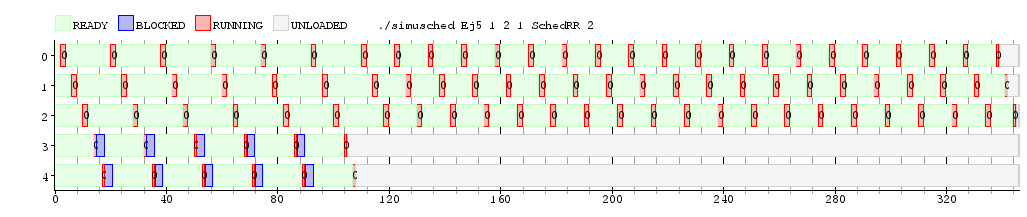
\includegraphics[width=450pt]{./Test/ej5_2.png}
	{$Lote 1$ - Scheduler RR - 1 core - 2 quantum}	
 
\end{center}

\begin{center}
  	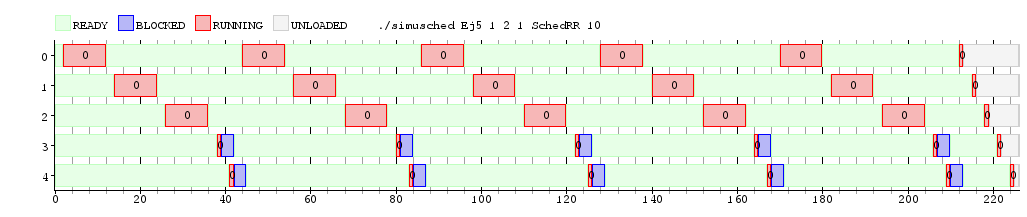
\includegraphics[width=450pt]{./Test/ej5_10.png}
	  {$Lote 1$ - Scheduler RR - 1 core - 10 quantum}	
\end{center}

\begin{center}
  	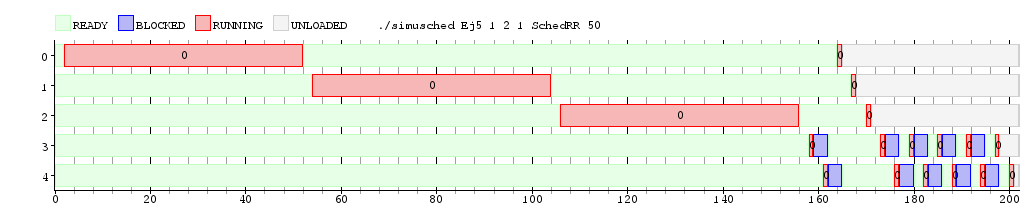
\includegraphics[width=450pt]{./Test/ej5_50.png}
	  {$Lote 1$ - Scheduler RR - 1 core - 50 quantum}	
\end{center}

\indent Se puede observar el cambio de tareas cíclico tanto porque terminaron su quantum o porque se bloquearon.\\


\indent Luego de estos experimentos pudimos observar ciertos puntos del comportamiento del Round-Robin:\\
\begin{itemize}
\item  Carácter circular del algoritmo.
\item  Desalojo de las tareas cuando se bloquean o terminan y la inmediata asignación del núcleo a la siguiente tarea en caso de existir alguna.
\item  Libre de inanición.
\item  Una tarea bloqueada es ignorada por el scheduler hasta que se desbloquee.
\end{itemize}

\indent Finalmente, dado su carácter circular y equitativo, podemos afirmar que todas las tareas que 
estén en condiciones de correr serán ejecutadas y ninguna será negada de tiempo de procesamiento.\\


\subsubsection[Resolución Ejercicio 5]{Ejercicio 6}

\subsubsection[Resolución Ejercicio 5]{Ejercicio 7}

\subsubsection[Resolución Ejercicio 8]{Ejercicio 8}

EN ESTE SOLO FALTARIA DECIR EL CASO REAL TRATANDO DE USAR NUESTRO LOTE YA HECHO

La idea principal de esta nueva versión de $Round-Robin$ se centraliza en que no permita migración entre
cores, esto se basa principalmente en utilizar una cola para cada núcleo por separado, y en cada
cola respectiva se encolaran las tareas que fueron asignadas inicialmente a cada nucleo.\\
Para desarrollar este tipo de algoritmo, el cual denominaremos $RR2$, utilizamos estructuras
puntuales, enunciadas a continuación:\\
\begin{itemize}
 \item Un vector $quantum$ y otro $quantumActual$, los cuales siguen cumpliendo la misma funcion que
 en Round-Robin 1.
 \item Un vector de colas denominado $colas$, en el cual, en la posición $i$ encontraremos la cola correspondiente
 a ese núcleo de procesamiento.
 \item Un diccionario de $Bloqueados$, donde la clave contendra el número de core, y en definición
 la tareas bloqueadas de ese core. Esto nos beneficiara cuando haya que reubicarla en la cola de procesos ready.
 \item Un vector de enteros $cantidad$, que como la palabra lo define, tendrá en cada posición $i$ 
 la totalidad de las tareas, ya sea bloqueadas, activas o en estado ready que tiene asignado ese core, beneficiandonos
 la determinación del núcleo al que se le asignará la tarea al momento de cargarla.
\end{itemize}
Cuando se carga una tarea, previamente, se chequeará que core tiene menor cantidad de procesos totales asignados (
aqui es donde el vector $cantidad$ entra en juego). Una vez que se obtiene este nucleo, se agrega 
la tarea a la cola correspondiente y se actualiza la cantidad sumando una unidad.\\
\indent Al bloquearse un proceso, se define una nueva entrada en el diccionario $bloqueados$ con el
pid y el nucleo correspondiente. De esta forma, al desbloquearse, colocamos la tarea en la cola del core
correspondiente y eliminamos la entrada del diccionario. Así logramos resolver el inconveniente de la nula
migración entre nucleos.\\
\indent Finalmente, cuando una tarea finaliza, la quitamos y descontamos una unidad a la posición $i$ del vector
$cantidad$. Esta es la única vez, en la cual se descuenta. Aunque una tarea se bloquee, la misma
seguirá contando en el vector. De esta forma se cumplirá, que las tareas son asignadas a los cores
con menor cantidad de tareas.\\
Luego de realizar dicha implementación, en comparación al Round-Robin original, hemos conjeturado 
las siguientes hipótesis:

\begin{enumerate}
 \item Dados un mismo lote de tareas y una misma configuración del scheduler (mismos costo en cambio
de contexto y quantum) un único núcleo de procesamiento, ambos algoritmos deben comportarse
de la misma manera.
\item Comportamiento menos eficiente en el RR2 con respecto al paralelismo, ya que al no permitir
migración de nucleos este se pierde.
\item Comportamiento más eficiente en el RR2 con lotes de tareas que se bloquean un gran numero
de veces. Esto surge ya que el Round-Robin original, es mas proclive a realizar cambios de contexto con la posibilidad
de darse un cambio de core.
\end{enumerate}

Por consiguiente, procederemos a demostrar lo conjeturado.\\

Iniciando con nuestra primer conjetura:\\

\textbf{Dados un mismo lote de tareas y una misma configuración del scheduler 
 (mismos costo en cambio de contexto y quantum)
un único núcleo de procesamiento, ambos algoritmos deben comportarse
de la misma manera.}\\

Trabajando con el lote que mencionamos a continuación:
    
    \begin{verbatim}
                                     TaskCPU 70
                                     TaskConsola 2 4 5
                                     TaskCPU 40
                                     TaskConsola 3 2 3
                                     TaskCPU 30
    \end{verbatim}

Utilizando un $quantum$ igual a 5 y un cambio de contexto igual a 1 obtuvimos 
resultados muy marcados, viendose notoriamente lo que queremos demostrar.\\

\begin{center}
    	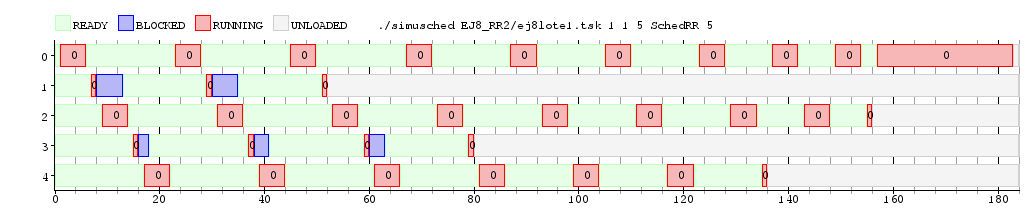
\includegraphics[width=450pt]{./EJ8_RR2/dif1corerr.png}
	{$Lote 1$ - Round Robin - 1 core - Quantum = 5 - cambio de contexto = 1}	
 \end{center}
 
 \begin{center}
    	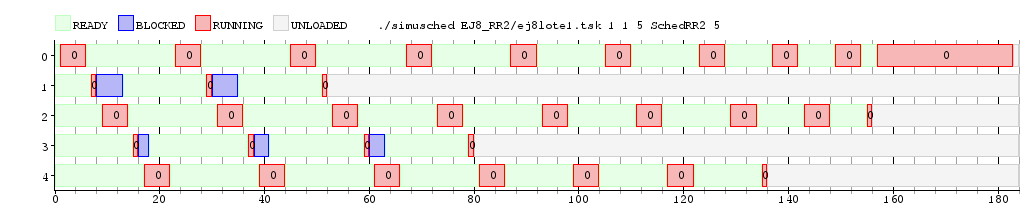
\includegraphics[width=450pt]{./EJ8_RR2/dif1corerr2.png}
	{$Lote 1$ - Round Robin 2 - 1 core - Quantum = 5 - cambio de contexto = 1}	
 \end{center}

Continuando con un lote distinto para ser mas precisos:

 \begin{verbatim}
                                     TaskCPU 70
                                     TaskConsola 5 6 7
                                     TaskCPU 40
                                     TaskConsola 10 9 8
                                     TaskCPU 30
 \end{verbatim}
 
Llegamos a lo siguiente:\\

 \begin{center}
    	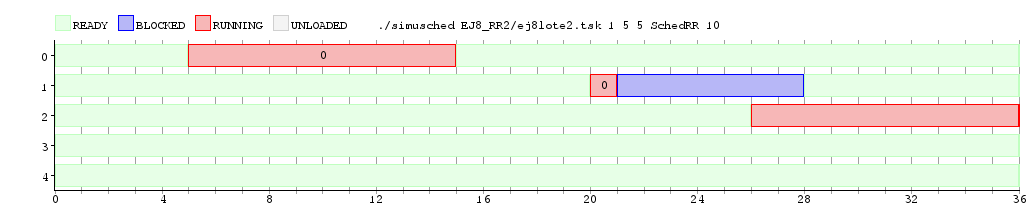
\includegraphics[width=450pt]{./EJ8_RR2/dif2corerr.png}
	{$Lote 2$ - Round Robin - 1 core - Quantum = 10 - cambio de contexto = 5}	
 \end{center}
 
 \begin{center}
    	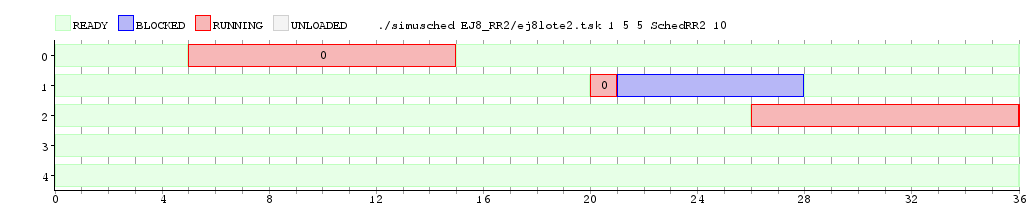
\includegraphics[width=450pt]{./EJ8_RR2/dif2corerr2.png}
	{$Lote 2$ - Round Robin 2 - 1 core - Quantum = 10 - cambio de contexto = 5}	
 \end{center}
 
 Viendose nuevamente, la igualdad que mencionamos. Hemos podido ver a su vez, que la única
 forma en la que los resultados sean distintos con el mismo lote seria modificando o la
 cantidad de $quantum$ o la unidad de cambio de contexto entre uno y otro.\\
 
 Aqui, un ejémplo para mayor precisión:\\
 
  \begin{center}
    	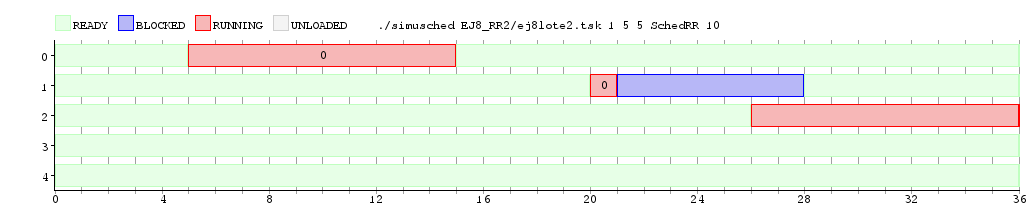
\includegraphics[width=450pt]{./EJ8_RR2/dif3corerr.png}
	{$Lote 2$ - Round Robin - 1 core - Quantum = 10 - cambio de contexto = 5}	
 \end{center}
 
 \begin{center}
    	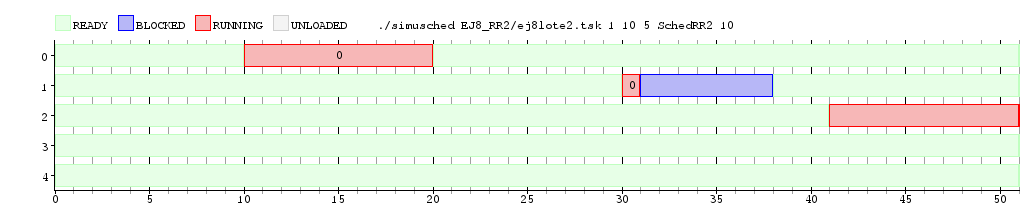
\includegraphics[width=450pt]{./EJ8_RR2/dif3corerr2.png}
	{$Lote 2$ - Round Robin 2 - 1 core - Quantum = 10 - cambio de contexto = 10}	
 \end{center}
 
 Concluimos entonces que, al trabajar con colas globales o no, utilizando un único núcleo y
 mismo lote quantum y cambio de contexto, ambos schedulers se comportan de la misma
 manera.\\
 
 Procedemos a demostrar la segunda conjetura:\\
 
 \textbf{Comportamiento menos eficiente en el RR2 con respecto al paralelismo, ya que al no permitir
migración de núcleos este lo pierde}\\

Para demostrar esta conjetura trabajamos con procesos que demanden mas uso del cpu como 
lo son las $taskCPU$\\

Un ejemplo de los lotes utilizados fue el siguiente:\\

\begin{verbatim}
                                     TaskCPU 40
                                     TaskCPU 15
                                     TaskCPU 50
                                     TaskCPU 30
                                     TaskCPU 50
\end{verbatim}

Obteniendo los siguientes datos relevantes:\\

\begin{center}
    	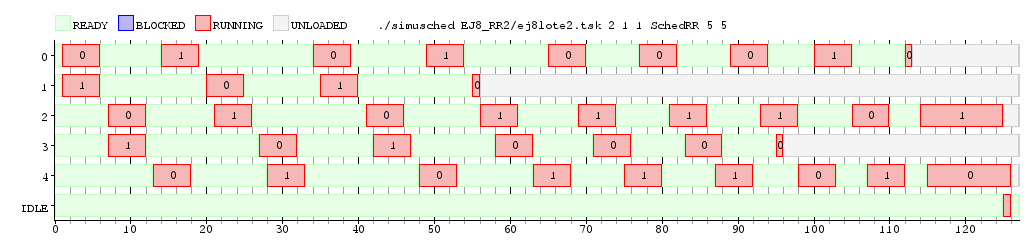
\includegraphics[width=450pt]{./EJ8_RR2/dif10corerr.png}
	{$Lote 3$ - Round Robin - 2 core - Quantum = 5 - cambio de contexto = 1}	
 \end{center}
 
 \begin{center}
    	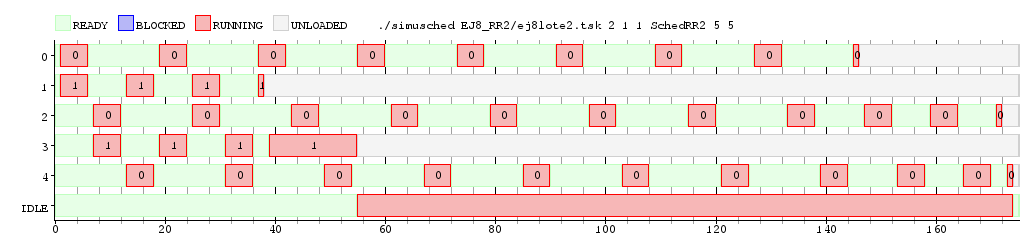
\includegraphics[width=450pt]{./EJ8_RR2/dif10corerr2.png}
	{$Lote 3$ - Round Robin 2 - 2 core - Quantum = 5 - cambio de contexto = 1}	
 \end{center}
 
 Se puede ver en estos diagramas como la implementación del Round Robin original trabaja
 mejor finalizando la ejecución de las tareas hasta 50 milisegundos antes.\\
 Esto se da por la falta de paralelismo de el RR2 ya que al ser asignados los procesos
 a cada core, cuando uno de los dos finaliza, este queda ocioso ya que no existe la
 posibilidad de migrar  procesos.\\
 
 Por ultimo, nuestra tercer y ultima conjetura:\\
 
 \textbf{Comportamiento mas eficiente en el RR2 con lotes de tareas que se bloquean un gran numero
de veces}

Para esta conjetura, trabajamos con lotes de tareas que utilicen el CPU y se bloqueen muchas
veces para poder demostrar la mejor performance del RR2.\\

A continuación un ejemplo, con el siguiente lote:

\begin{verbatim}
                                     TaskCPU 40
                                     TaskBatch 10  5
                                     TaskCPU 50
                                     TaskBatch 15 8
                                     TaskCPU 10

\end{verbatim}


   \begin{center}
    	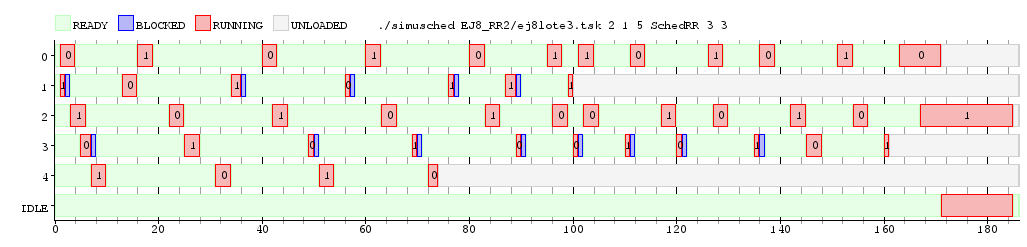
\includegraphics[width=450pt]{./EJ8_RR2/dif5corerr.png}
	{$Lote 3$ - Round Robin - 2 core - Quantum = 3 - cambio de contexto = 1}	
 \end{center}
 
 \begin{center}
    	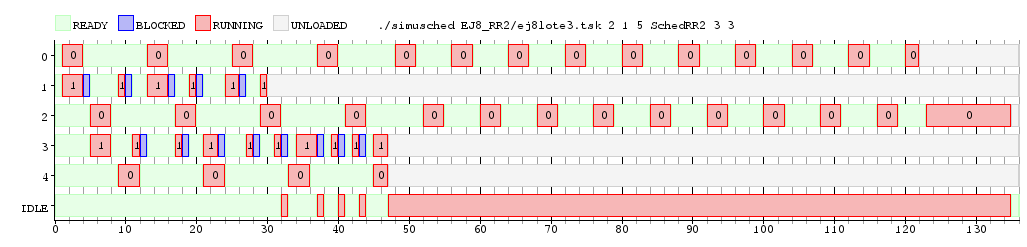
\includegraphics[width=450pt]{./EJ8_RR2/dif5corerr2.png}
	{$Lote 3$ - Round Robin 2 - 2 core - Quantum = 3 - cambio de contexto = 1}	
 \end{center}

 Se puede observar por los diagramas como el RR2 tiene una mejor performance en este estilo
 de lotes llegando a finalizar las ejecuciones hasta 50 milisegundos antes que el Round-Robin
 original.\\
 Como el Round-Robin original tiene pérdida de tiempo con el cambio de contexto y
 migración de tareas este empeora su performance en comparación al RR2 que no admite
 este tipo de migración es notorio la superioridad en relación a nuestra conjetura.\\
 
 Podemos concluir luego de estas demostraciones que, el Round-Robin original es ampliamente
 superior desde el punto de vista de la performance que se obtiene al trabajar con tareas
 que demanden mucho uso del CPU, mientras que el RR2 es ampliamente mejor cuando se utilicen
 tareas que se bloqueen por un tiempo considerable.\\
 

